

% This is "sig-alternate.tex" V1.9 April 2009
% This file should be compiled with V2.4 of "sig-alternate.cls" April 2009
%
% This example file demonstrates the use of the 'sig-alternate.cls'
% V2.4 LaTeX2e document class file. It is for those submitting
% articles to ACM Conference Proceedings WHO DO NOT WISH TO
% STRICTLY ADHERE TO THE SIGS (PUBS-BOARD-ENDORSED) STYLE.
% The 'sig-alternate.cls' file will produce a similar-looking,
% albeit, 'tighter' paper resulting in, invariably, fewer pages.
%
% ----------------------------------------------------------------------------------------------------------------
% This .tex file (and associated .cls V2.4) produces:
%       1) The Permission Statement
%       2) The Conference (location) Info information
%       3) The Copyright Line with ACM data
%       4) NO page numbers
%
% as against the acm_proc_article-sp.cls file which
% DOES NOT produce 1) thru' 3) above.
%
% Using 'sig-alternate.cls' you have control, however, from within
% the source .tex file, over both the CopyrightYear
% (defaulted to 200X) and the ACM Copyright Data
% (defaulted to X-XXXXX-XX-X/XX/XX).
% e.g.
% \CopyrightYear{2007} will cause 2007 to appear in the copyright line.
% \crdata{0-12345-67-8/90/12} will cause 0-12345-67-8/90/12 to appear in the copyright line.
%
% ---------------------------------------------------------------------------------------------------------------
% This .tex source is an example which *does* use
% the .bib file (from which the .bbl file % is produced).
% REMEMBER HOWEVER: After having produced the .bbl file,
% and prior to final submission, you *NEED* to 'insert'
% your .bbl file into your source .tex file so as to provide
% ONE 'self-contained' source file.
%
% ================= IF YOU HAVE QUESTIONS =======================
% Questions regarding the SIGS styles, SIGS policies and
% procedures, Conferences etc. should be sent to
% Adrienne Griscti (griscti@acm.org)
%
% Technical questions _only_ to
% Gerald Murray (murray@hq.acm.org)
% ===============================================================
%
% For tracking purposes - this is V1.9 - April 2009

\documentclass{sig-alternate}
  \pdfpagewidth=8.5truein
  \pdfpageheight=11truein

\usepackage[latin1]{inputenc}
\usepackage{graphicx}
\usepackage{color}
\usepackage{url}
\usepackage[english]{babel}

\begin{document}
%
% --- Author Metadata here ---
\conferenceinfo{SAC'14}{March 24-28, 2014, Gyeongju, Korea.}
\CopyrightYear{2014} % Allows default copyright year (2002) to be over-ridden - IF NEED BE.
\crdata{978-1-4503-2469-4/14/03}  % Allows default copyright data (X-XXXXX-XX-X/XX/XX) to be over-ridden.
% --- End of Author Metadata ---

\title{MUSES: A corporate user-centric system which applies computational intelligence methods}
%\subtitle{[Poster paper]}
%
% You need the command \numberofauthors to handle the 'placement
% and alignment' of the authors beneath the title.
%
% For aesthetic reasons, we recommend 'three authors at a time'
% i.e. three 'name/affiliation blocks' be placed beneath the title.
%
% NOTE: You are NOT restricted in how many 'rows' of
% "name/affiliations" may appear. We just ask that you restrict
% the number of 'columns' to three.
%
% Because of the available 'opening page real-estate'
% we ask you to refrain from putting more than six authors
% (two rows with three columns) beneath the article title.
% More than six makes the first-page appear very cluttered indeed.
%
% Use the \alignauthor commands to handle the names
% and affiliations for an 'aesthetic maximum' of six authors.
% Add names, affiliations, addresses for
% the seventh etc. author(s) as the argument for the
% \additionalauthors command.
% These 'additional authors' will be output/set for you
% without further effort on your part as the last section in
% the body of your article BEFORE References or any Appendices.


\numberofauthors{4} %  in this sample file, there are a *total*
% of EIGHT authors. SIX appear on the 'first-page' (for formatting
% reasons) and the remaining two appear in the \additionalauthors section.
%
\author{
% You can go ahead and credit any number of authors here,
% e.g. one 'row of three' or two rows (consisting of one row of three
% and a second row of one, two or three).
%
% The command \alignauthor (no curly braces needed) should
% precede each author name, affiliation/snail-mail address and
% e-mail address. Additionally, tag each line of
% affiliation/address with \affaddr, and tag the
% e-mail address with \email.
%
% 1st. author
\alignauthor
A.M. Mora, P. De las Cuevas, J.J. Merelo\\
%\titlenote{Dr.~Trovato insisted his name be first.}\\
       \affaddr{Departamento de ATC}\\
%       \affaddr{ETSIIT-CITIC}\\
       \affaddr{University of Granada}\\
%       \email{{\footnotesize \{amorag,paloma,jmerelo\}@geneura.ugr.es}}
% 2nd. author
\alignauthor 
S. Zamarripa, M. Juan,\\ A.I. Esparcia-Alc�zar\\
%\titlenote{The secretary disavows
%any knowledge of this author's actions.}\\
       \affaddr{S2 Grupo}\\
%       \affaddr{P.O. Box 1212}\\
%       \affaddr{Dublin, Ohio 43017-6221}\\
%       \email{\{aesparcia,szamarripa\}@s2grupo.es}
\and
% 3rd. author
\alignauthor 
M. Burvall, H. Arfwedson\\
%\titlenote{This author is the
%one who did all the really hard work.}\\
       \affaddr{Sweden Connectivity}\\
%       \affaddr{1 Th{\o}rv{\"a}ld Circle}\\
%       \affaddr{Hekla, Iceland}\\
%       \email{\{markus,henrik\}@sconnectivity.com}
%\and  % use '\and' if you need 'another row' of author names
% 4th. author
\alignauthor 
Z. Hodaie\\
       \affaddr{HITEC}\\
       \affaddr{University of Hamburg}
%       \affaddr{P.O. Box 5000}\\
%       \email{hoitate@hitec.com}
% 5th. author
%\alignauthor Sean Fogarty\\
%       \affaddr{NASA Ames Research Center}\\
%       \affaddr{Moffett Field}\\
%       \affaddr{California 94035}\\
%       \email{fogartys@amesres.org}
% 6th. author
%\alignauthor Charles Palmer\\
%       \affaddr{Palmer Research Laboratories}\\
%       \affaddr{8600 Datapoint Drive}\\
%       \affaddr{San Antonio, Texas 78229}\\
%       \email{cpalmer@prl.com}
}
% There's nothing stopping you putting the seventh, eighth, etc.
% author on the opening page (as the 'third row') but we ask,
% for aesthetic reasons that you place these 'additional authors'
% in the \additional authors block, viz.
%>>>\additionalauthors{Additional authors: John Smith (The
%Th{\o}rv{\"a}ld Group, email: {\texttt{jsmith@affiliation.org}})
%and Julius P.~Kumquat (The Kumquat Consortium, email:
%{\texttt{jpkumquat@consortium.net}}).}
%\date{30 July 1999}
% Just remember to make sure that the TOTAL number of authors
% is the number that will appear on the first page PLUS the
% number that will appear in the \additionalauthors section.


\maketitle
\begin{abstract}
This work presents the description of the architecture of a novel enterprise security system, still in development, which can prevent and deal with the security flaws derived from the users in a company. Thus, the Multiplatform Usable Endpoint Security system (MUSES) considers diverse factors such as the information distribution, the type of accesses, the context where the users are, the category of users, or the mix between personal and private data, among others.
This system includes an event correlator and a risk and trust analysis engine to perform the decision process. MUSES follows a set of defined security rules, according to the enterprise security policies, but it is able to self-adapt the decisions and even create new security rules depending on the user behaviour, the specific device, and the situation or context. To this aim MUSES applies machine learning and computational intelligence techniques which can also be used to predict potential unsafe or dangerous user's behaviour.
\end{abstract}

%A category including the fourth, optional field follows...
\category{C.0}{Computer Systems Organization}{GENERAL}
% A category with the (minimum) three required fields
\category{K.6.5}{Computing Milieux}{MANAGEMENT OF COMPUTING AND INFORMATION SYSTEMS}[Security and Protection]

\terms{Security}

\keywords{Enterprise security, Multiplatform, User-centric system, BYOD, Self-adaptation, Event Correlation, Risk and Trust analysis, Security Policies}

%
%%%%%%%%%%%%%%%%%%%%%%%%%%%%%%%   INTRODUCTION   %%%%%%%%%%%%%%%%%%%%%%%%%%%%%%%
%
\section{Introduction}
\label{sec:intro}

Some years ago, company data were stored in own servers which were accessed by the employees or users by means of desktop or portable computers. Nowadays it is frequent that these data are distributed among multiple machines, even not all belonging to the company, and being consulted and modified through a wide amount of devices, some of them owned by the company's users. This is the so-called Bring Your Own Device (BYOD) philosophy. It is becoming highly successful due to the impact that smartphones and tablets are having in the market.
Data security and privacy are key factors for a company, thus, to protect them, it is usual to define Organisational Security Policies. Their definition is nowadays a very difficult problem, since the BYOD tendency means that several factors must be considered \cite{Opp_Security11}, most of them previously ignored or non-considered in the security systems, for instance the current mixture between personal and professional information in these devices (the user could navigate inside social networks where there could be friends and also company partners or clients).

Moreover, it has been demonstrated that people are the main hazard regarding the company security \cite{Adams_Users05}, so in this situation, some monitorization and security-aimed applications are arising. Most of them try to be non-intrusive (regarding the users' personal data), friendly and easy to manage.

This work presents the general architecture of one of these systems, named MUSES, Multiplatform Usable Endpoint Security system. It is being implemented inside an European Project and will provide a device independent, user-centric, and self-adaptive corporate security system, able to cope with the concept of seamless working experience on different devices. This concept is a methodology of work which allows users to start/continue a working session over multiple devices and locations without any significant loss of data. This new situation has a big impact from the point of view of the security \cite{Schu_SecPatterns05}, since the company's data borders have changed in the last years so now the users can access significant data from outside the enterprise, and possibly through a non absolutely secure channel.

In this scenario MUSES will analyse the users' behaviour and predict, using computational intelligence methods, risky or dangerous actions regarding both an event correlation and a risk and trust analysis engines. The system will be able to learn from the past user's behaviour, and react in a non-intrusive way to the potentially dangerous sequence of actions that he or she is conducting at any time.

The rest of the paper is organised as follows: next section gives a brief overview on the MUSES system initial proposal. Then, the designed architecture is deeply described in Section \ref{sec:architecture}. Finally, in Section \ref{sec:advantages} MUSES features are compared with other existing products, giving an idea on its advantages, along with the advances beyond the state of the art that this system aims to.

%
%%%%%%%%%%%%%%%%%%%%%%%%%%%%   SYSTEM OVERVIEW   %%%%%%%%%%%%%%%%%%%%%%%%%%%%
%
\section{System initial overview}
\label{sec:system}

MUSES system will work as presented in Figure \ref{fig:system_overview}. The user interacts with the devices, own or corporate, through the MUSES graphical interface and inside his or her own context (situation, connection, status). This application includes two modules, a \textit{controller} and an \textit{actuator}. The first one monitorizes the environment (context) and the user's behaviour, translating his/her actions into a sequence of events. These events, along with the patterns defining the user's conduct, are processed by the system in real-time by means of a Risk and Trust Analysis Engine (RT2AE) and an Event Correlation module. Then, a decision is taken in the corporate security operations centre (SOC) side, considering the RT2AE output and the set of security rules adapted to that specific user and context. The corresponding feedback is communicated to the user through the \textit{actuator}, which is also in charge of triggering the recommended actions to stop the user's or application's doings, in case it is required.


%This client contains a \textit{monitorization module}, which gathers the performed sequence of events and user context information; a \textit{controller module} in charge of take some light decisions considering the server response to the current situation (it will also take the control in case the device cannot connect with the server). The device controller will trigger the \textit{actuator} if necessary. This module will provide the user with some feedback, and will interact with the applications being monitorized if recommended or required.
%
% This application contains, in addition to an user interface to manage it, the main modules in the security-aimed decision process: the \textit{RT2AE} and the \textit{Event Correlator}. These components are connected between them and also with the main \textit{Controller}, that will connect with the device side sending the selected set of security rules that better fit with the current situation, along with the actions to be performed according to them.

%\begin{figure}
%\centering
%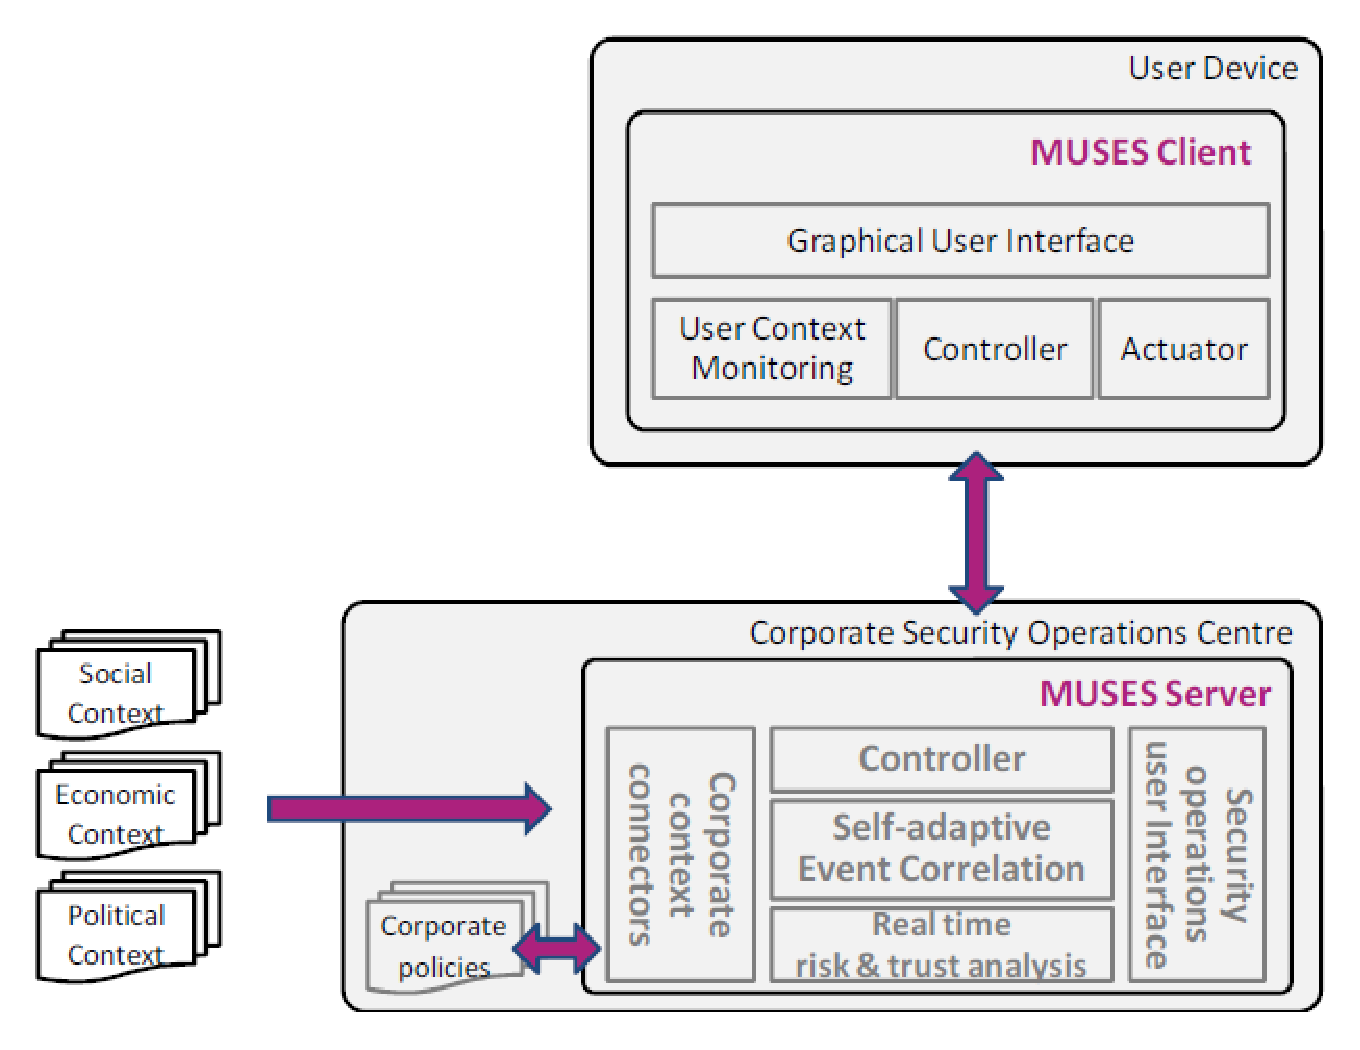
\epsfig{file=architecture.eps, scale=0.38}
%\caption{Proposed architecture\label{fig:architecture}}
%\end{figure}


\begin{figure*}[ht]
\centering
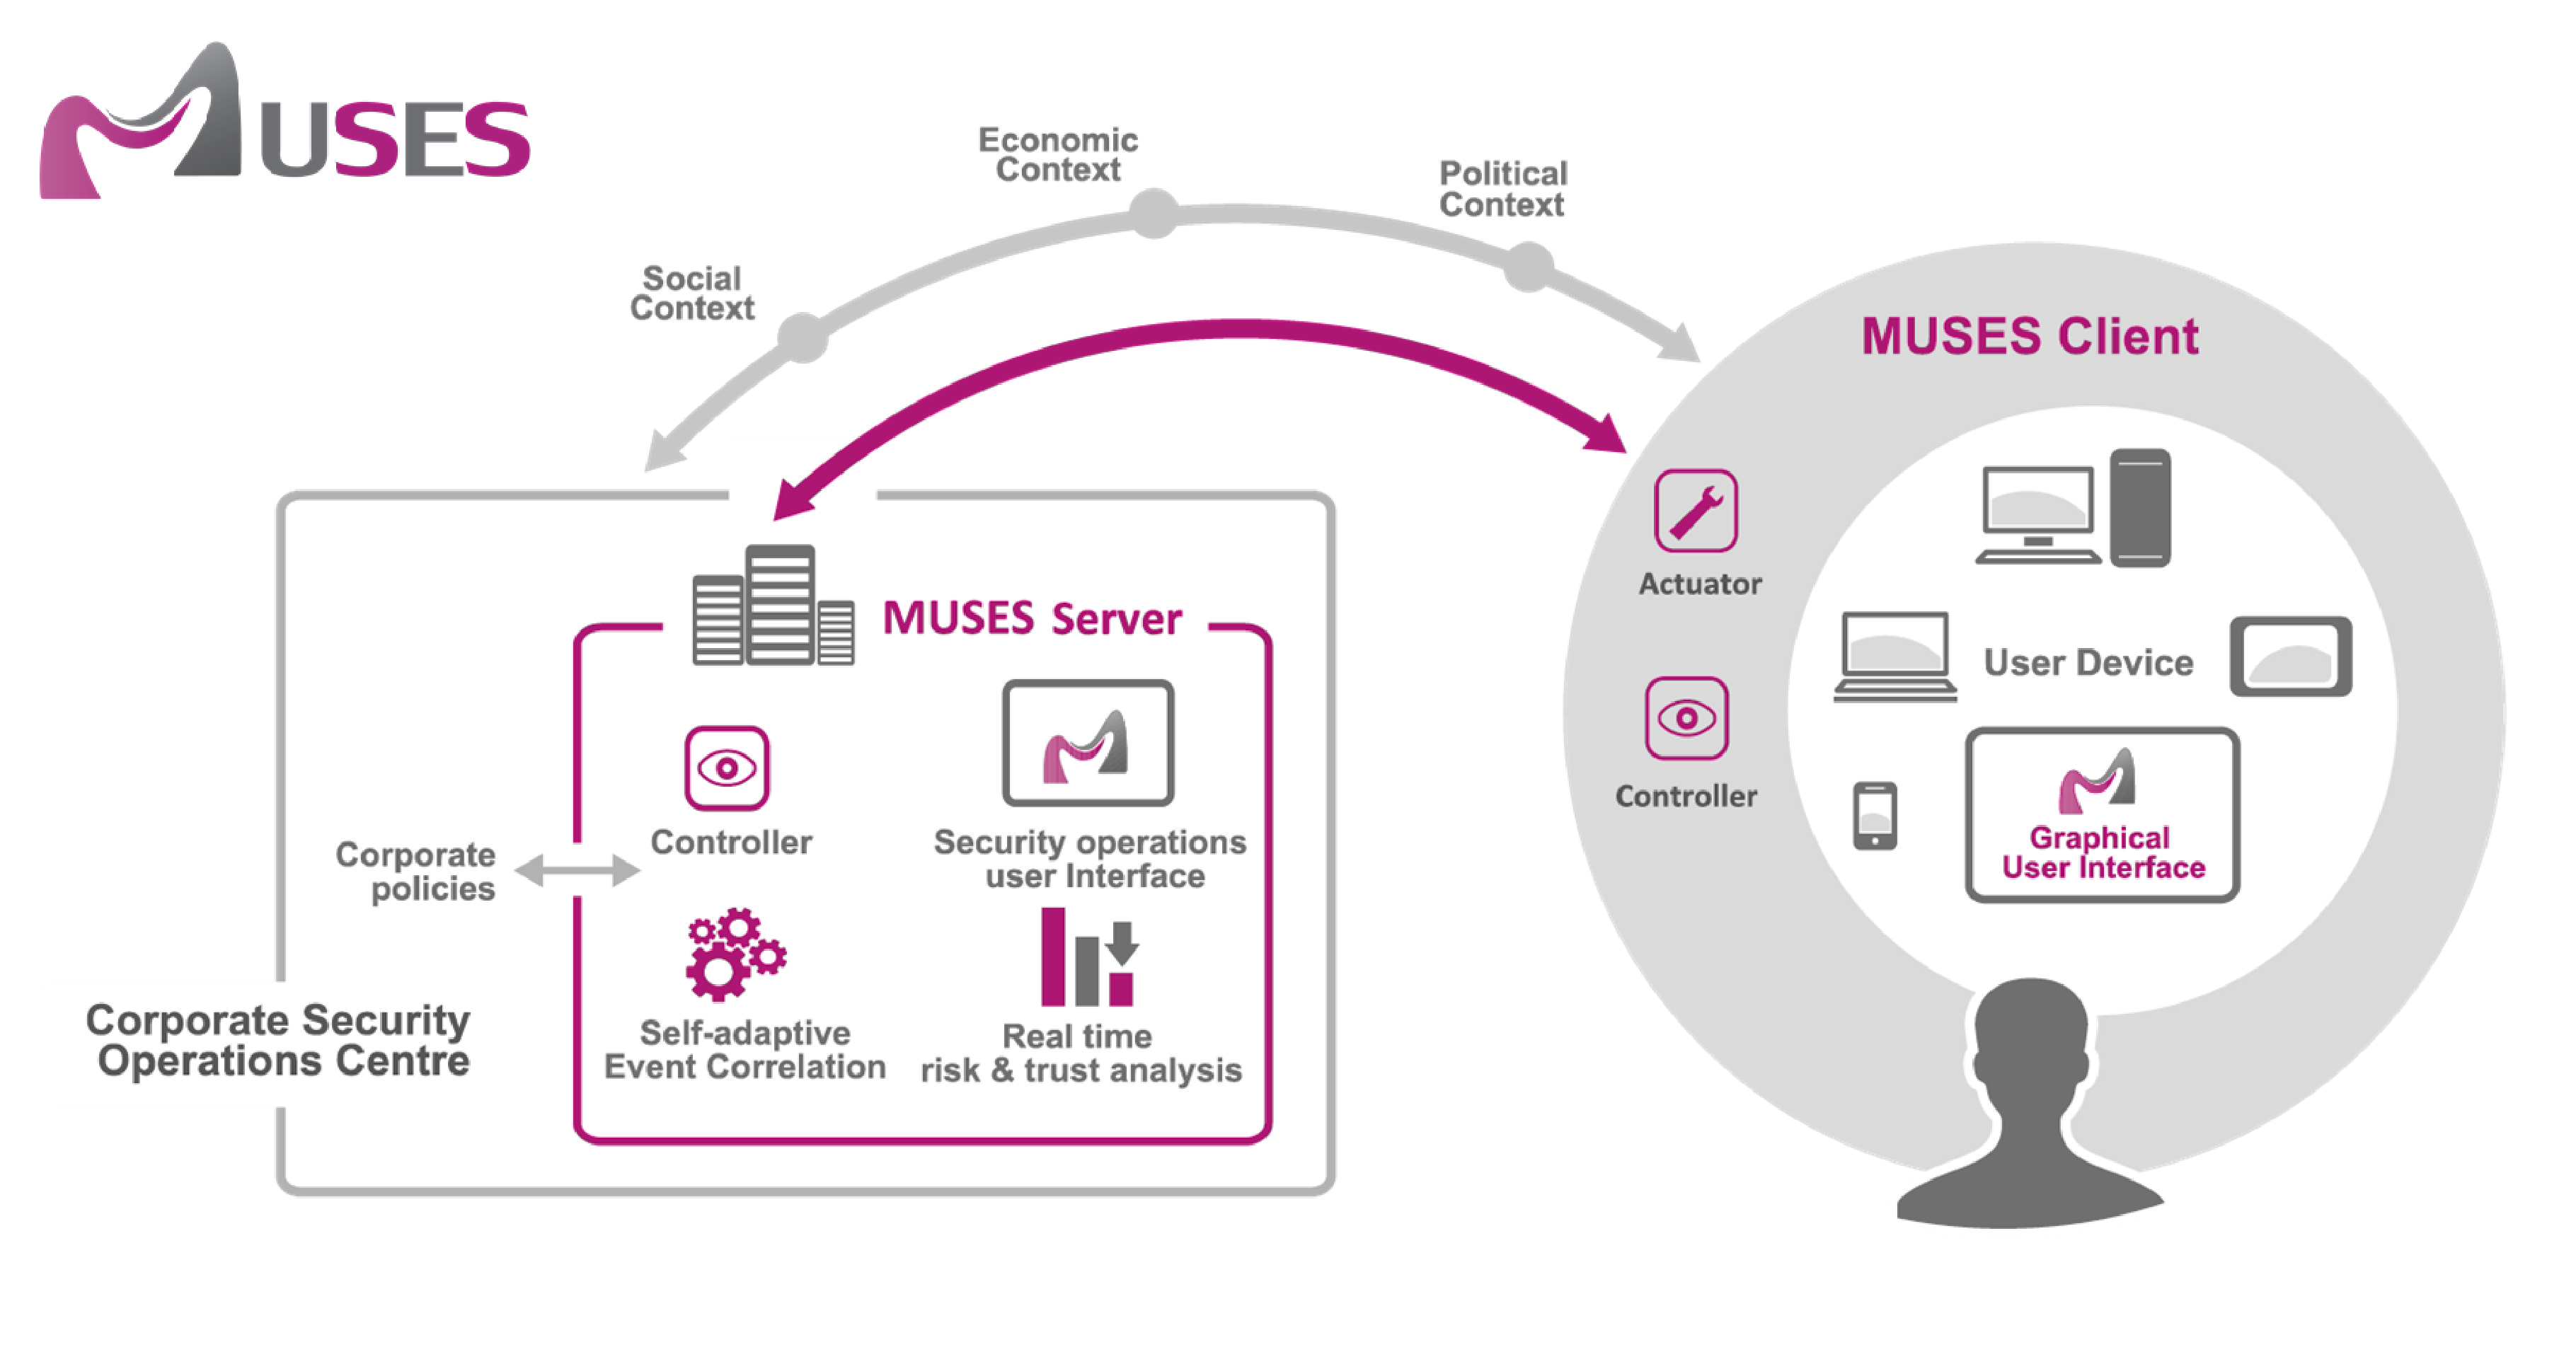
\epsfig{file=system_overview2.eps, scale=0.22}
\caption{MUSES system overview.\label{fig:system_overview}}
\end{figure*}

%\begin{figure*}[ht]
%\centering
%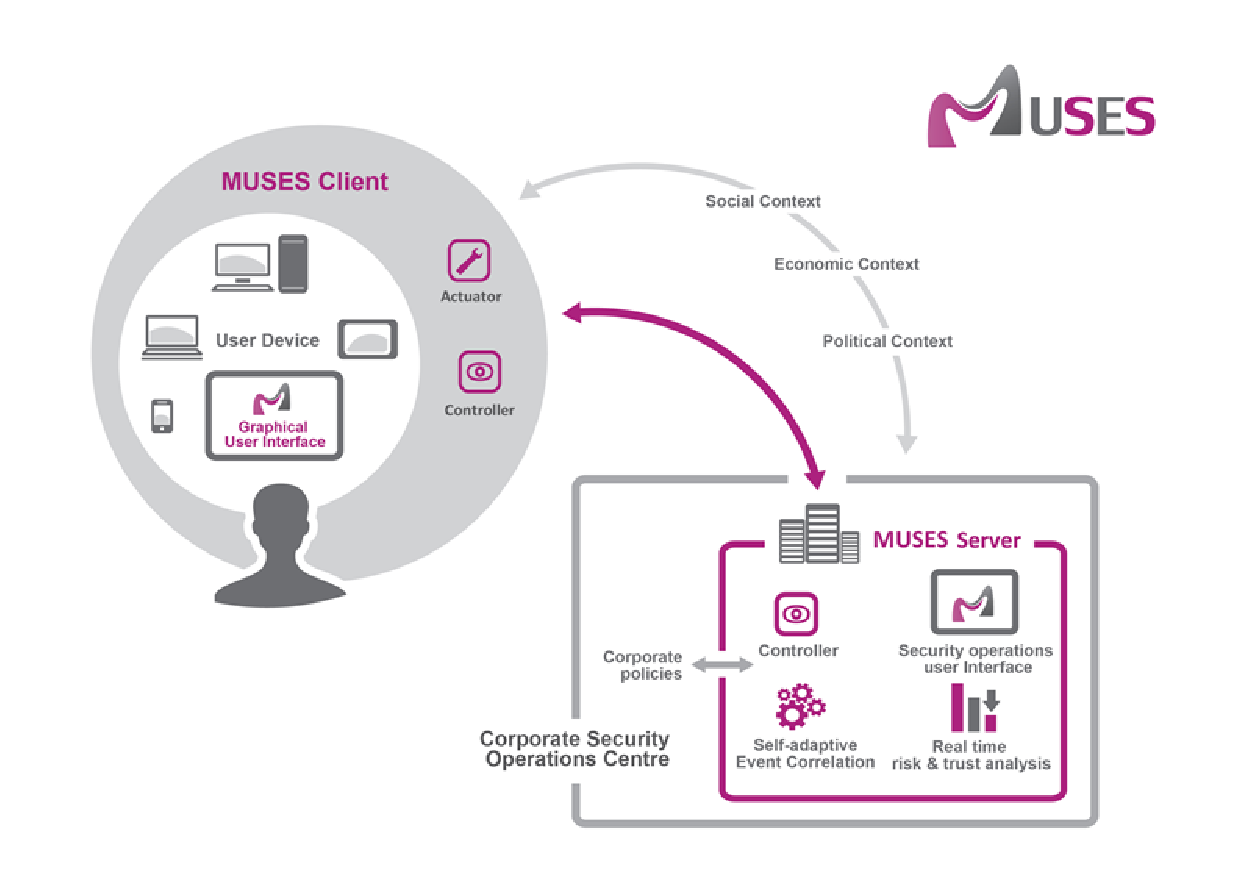
\epsfig{file=system_overview.eps, scale=0.5}
%\caption{MUSES system overview.\label{fig:system_overview}}
%\end{figure*}

%
%%%%%%%%%%%%%%%%%%%%%%%%%%%%   SYSTEM ARCHITECTURE   %%%%%%%%%%%%%%%%%%%%%%%%%%%
%
\section{MUSES Architecture}
\label{sec:architecture}


\begin{figure*}[ht]
\centering
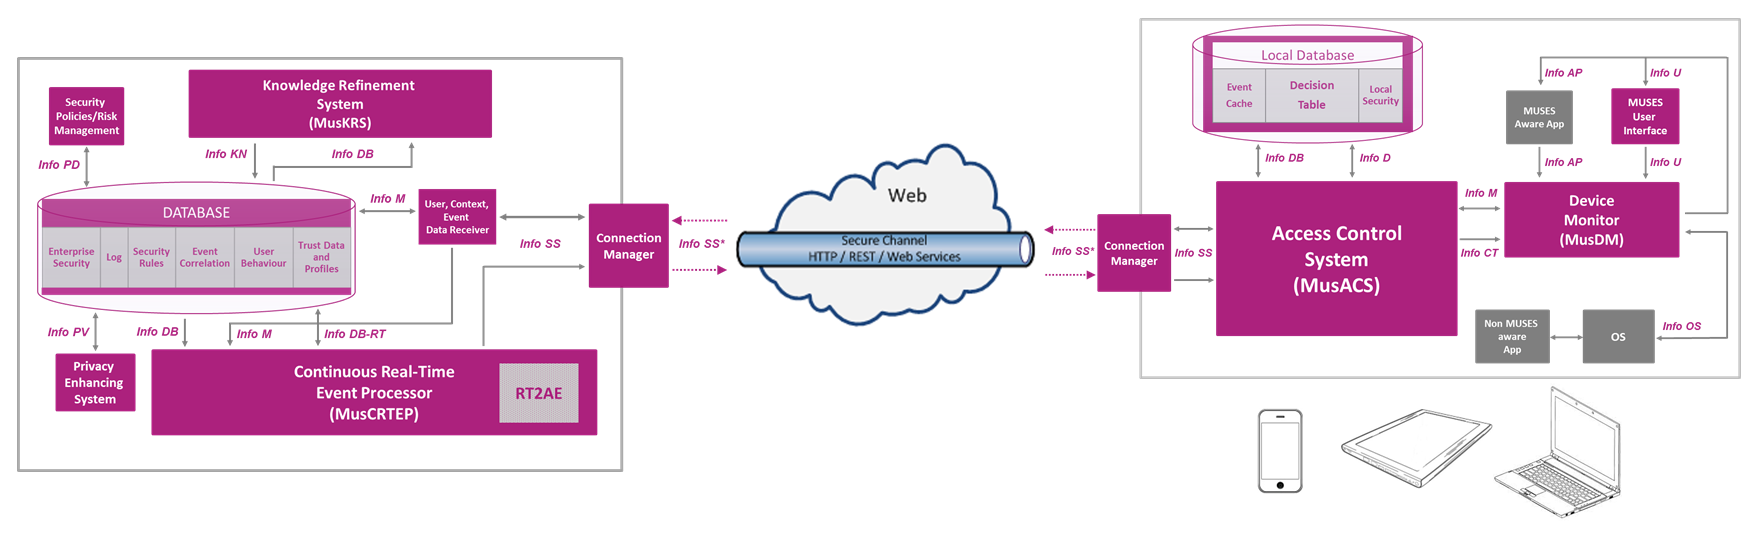
\epsfig{file=client_server_architecture.eps, scale=0.61}
\caption{MUSES Architecture Overview.\label{fig:client_server_architecture}}
\end{figure*}


The defined MUSES architecture is shown in Figure \ref{fig:client_server_architecture}. It is a \textit{client/server} approach in which the \textit{client} program will be installed in every user's mobile or portable device, independently of the platform (operating system and type of device). The \textit{server} side would be installed in the corporate SOC. Both sides are connected through a secure channel (using HTTPS) over Internet.

The rationale for this decision is based on two main reasons: 1) there is need for a high computational power in order to perform the event correlation and self-adaptation processes, so a quite powerful machine should be used (server); 2) there are two clearly separated parts in the system, namely the users (client) and the enterprise (server).

There are two working modes for every device in the system: online and offline. In the \textit{online} mode the device can connect with the MUSES server, so it can request the server to make a decision. On the other hand, in \textit{offline} mode the server cannot be reached by the device (there is not an available connection between them), so all the decisions should be made locally. Anyway, in this mode, the gathered information by the sensors in the device will be stored for later submission to the server side (when a connection is available), in order to be processed in the knowledge refinement process.

In that figure the high-level components in each part are shown. They are described in the following text.

% ----------------------------------------------

\subsection{Client/Device side}
\label{subsec:client}

Figure \ref{fig:client_submodules} shows the client architecture in detail, including the second-level components, and the information flows labelled as `Info XX'.

\begin{figure*}[ht]
\centering
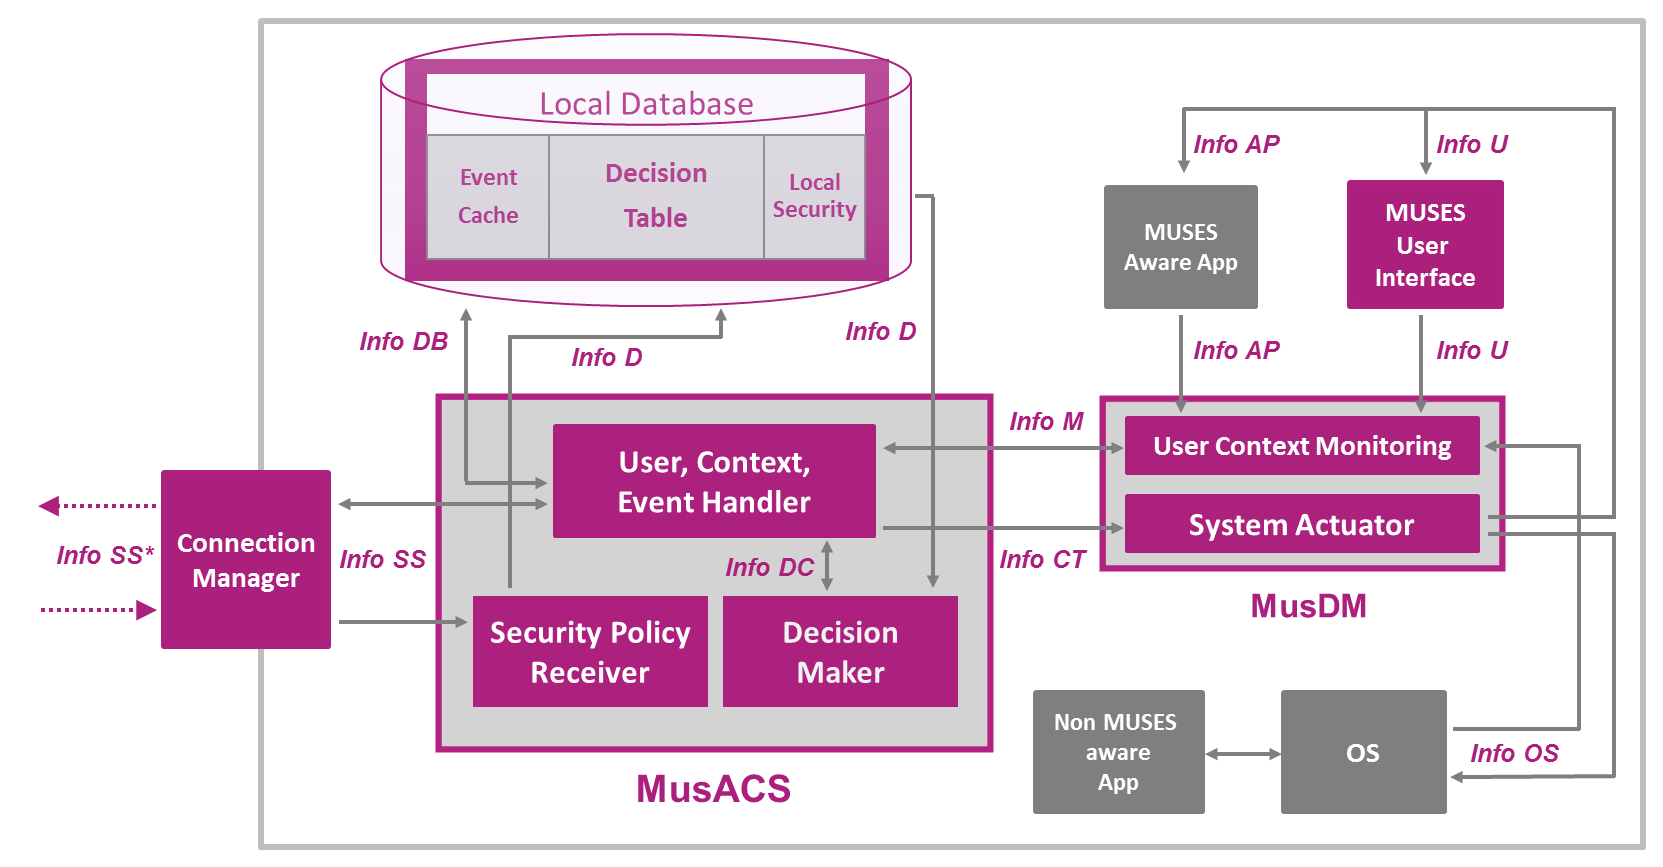
\epsfig{file=client_submodules.eps, scale=0.5}
\caption{MUSES Client Architecture (Submodules).\label{fig:client_submodules}}
\end{figure*}

There are three main components in this side:
\begin{itemize}
 	 \item \textit{Local Database}: it is a local security-based storage, which includes the set of security rules to be applied locally, user authentication data, and a cache of gathered events and information. The latter will be useful when the device is in offline mode, so these data are stored to be later submitted to the server side. It contains the so-called \textit{Decision Table}, a set of rules in which the antecedents are high-level events, and the consequents are the corresponding decisions/actions, namely `allow', `deny' or `request' (the decision must be made in the server side).
 	 \item \textit{Device Monitor (MusDM)}: module which gathers the events and information produced by the user. It also acts following the decisions made by the system, in order to allow or deny the controlled application (or the user) for doing something. As it can be seen in Figure \ref{fig:client_submodules}, it is composed by a monitoring and an actuator submodules.
 	 \item \textit{Access Control System (MusACS)}: module in charge of making the decisions considering the gathered data. These decisions can be made locally (if possible), or can be requested to the server (if there is no rule which matches with the occurred events). The subcomponents are the \textit{Decision Maker}, which performs the decision process; the \textit{User, Context, Event Handler}, which processes the events and information to be used for making the decision or stored for further submission (depending on the mode and on the gathered data); and the \textit{Security Policy Receiver} that updates the set of decisions (or Device Policies) in the Decision Table with those received from the server side, after an update or decision process.
\end{itemize}

The rest of the components are: the \textit{MUSES User Interface (UI)}, the application through which the user interacts with the system; and the \textit{Connection Manager} which controls the communications between client and server sides. 
In addition, there are two types of applications considered in this system: on the one hand the \textit{MUSES Aware App}, which is an application adapted to MUSES, so the system can directly interact with it (monitoring and acting). This application must be implemented using the MUSES API (Application Program Interface)\footnote{The MUSES API will be defined in the project, so for every application desired to be MUSES Aware, it should be implemented using this.}. On the other hand the \textit{Non MUSES Aware App} is that which MUSES cannot directly interact with. Usually it will be accessed through the operating system (OS).


% ----------------------------------------------

\subsection{Server side}
\label{subsec:server}

The server architecture can be seen in detail (at sub-module level) in Figure \ref{fig:server_submodules}, including as previously the information flows.

\begin{figure*}[ht]
\centering
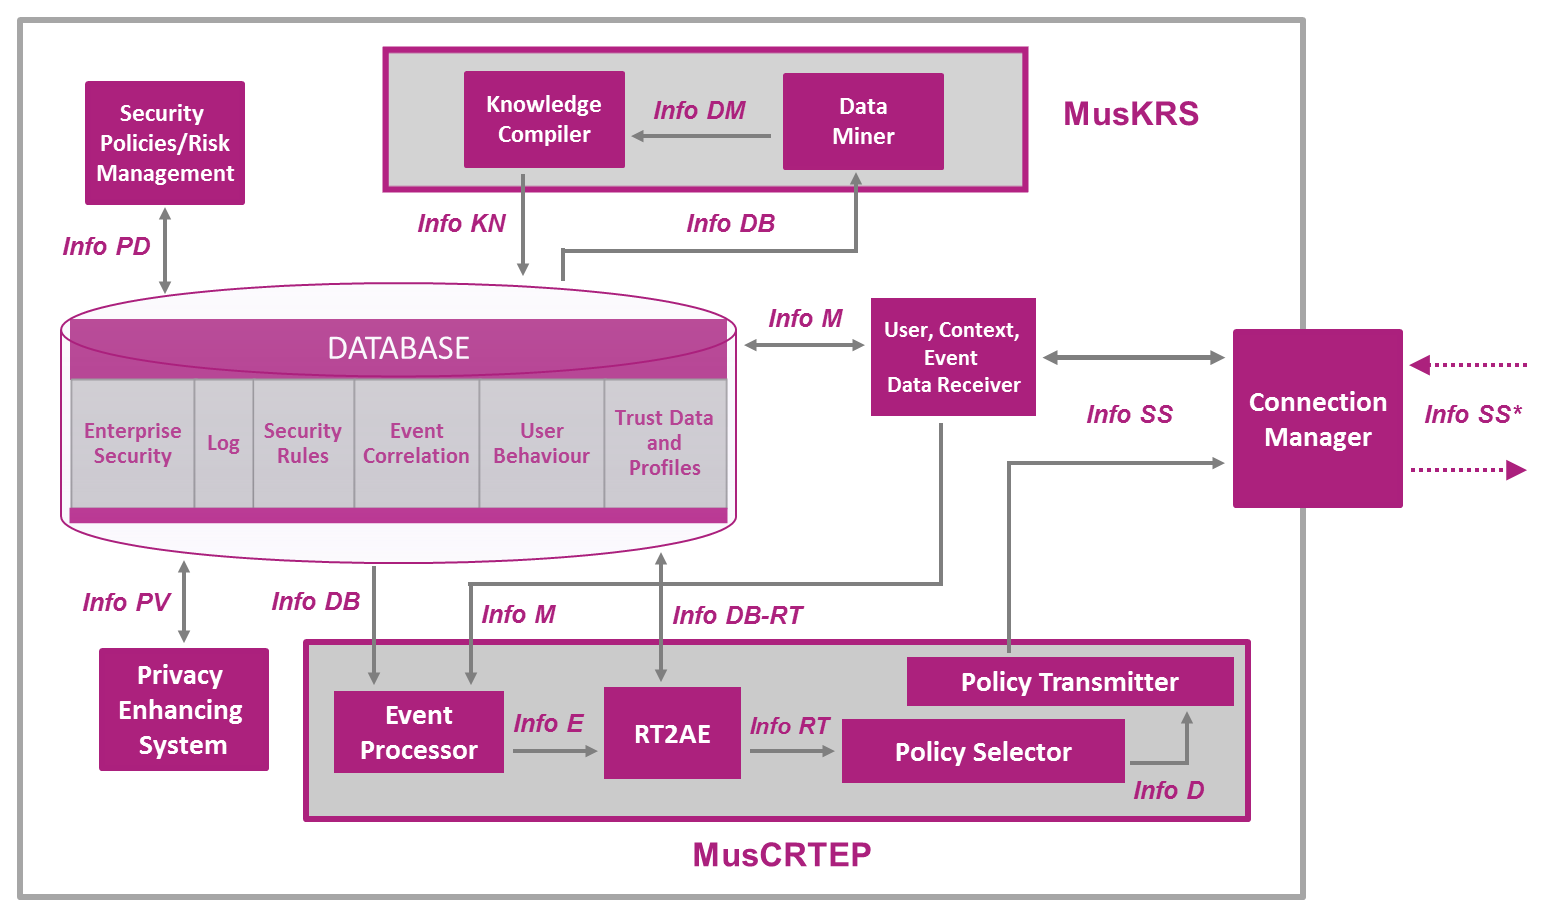
\epsfig{file=server_submodules.eps, scale=0.5}
\caption{MUSES Server Architecture (Submodules).\label{fig:server_submodules}}
\end{figure*}


As in the client, there are three main components:
\begin{itemize}
	 \item \textit{System Database}: it stores all the information that the system will manage, including authentication data, enterprise security policies, assets' values, user-related information (trust, context), events data, and, of course, security rules to apply (regarding the security policies).

	 \item \textit{Continuous Real-Time Event Processor (MusCRTEP)}: this component is the core of the MUSES system with respect to the decision making process. It includes an \textit{Event Processor}, the module in charge of performing the event correlation process \cite{EventProcessing_Luckham02,SurveyEventCorrelation_Tiffany02,EventProcessing_Luckham12}, gathering the set of occurred events and doing a rule-based threat identification. The output of this module is taken by the \textit{RT2AE}, which also considering information such as trust data and profiles, assets' values, user reputation, or opportunity, performs a risk and trust analysis task \cite{RT2AE_SOTICS13}, and extracts the set of potential rules to consider in the analysed situation. Then, these rules are transformed into decisions (or Device Policies) by the \textit{Policy Selector}, that are submitted to those devices to which they apply by the \textit{Policy Transmitter}.

	 \item \textit{Knowledge Refinement System (MusKRS)}: this module is in charge of analysing the information stored in the system database, identifying relevant data, such as important patterns, key features, or security incidents. These are later processed for tuning up the existing set of rules or for inferring new ones. 
%All this process is repeated asynchronously (sometimes a day, for instance) in order to adapt the security rules to new situations (predict user's behaviour).
\end{itemize}

There are some other components, namely: the \textit{Security Policies/Risk Management} tool, that lets the company's chief security officer (CSO) to define and manage Security Policies and Rules in a friendly way. It also lets the management of risk-related information, useful for the RT2AE process, such as the assets' values. The \textit{Privacy Enhancing System} which is a module aimed to fit with the legal compliance of the system regarding the user's data anonymisation. The \textit{User, Context, Event Data Receiver} is devoted to receive data from the device side (events, user-related, etc) and to distribute them among the components (storing in the database, and requesting the Event Processor to start the correlation task). Finally, there is another \textit{Connection Manager} which controls the communication with the device side.

As previously stated, one of the main features of the presented system will be the self-adaptation (to the user and context) of the set of security rules. To this end, the MusKRS's task will be run asynchronously to the system working. This process is composed by two steps: first, a Data Mining procedure \cite{DataMining_Lee01} will be performed, considering the whole amount of historic information mainly regarding user's behaviour and context. Some methods such as Clustering \cite{Clustering_Jain99,Clustering_Xu05} (grouping data), Pattern Recognition \cite{PatternMining_Han07} (usual situations identification), or Feature Selection \cite{FeatureSelection_Guyon03} (main variables/values in the data) will be applied. The second step consists in a refinement and inference process, performed by means of Machine Learning \cite{MachineLearning_Bishop06} and Computational Intelligence techniques. Regarding the latter, some methods will be used, such as Evolutionary or Genetic Algorithms \cite{EAs_Back96,GAs_Goldberg89} for parameters/values optimisation; or Genetic Programming \cite{GP_Koza92} for the modification of security rules.

Thus the set of rules will be adapted to every user in the system, updating some of the existing and creating new ones (always respecting the corporate security policies).
Moreover, some predictive models will be also obtained applying other soft computing techniques, so the user's potentially dangerous behaviour will be anticipated.

%\begin{table}
%\centering
%\caption{Frequency of Special Characters}
%\begin{tabular}{|c|c|l|} \hline
%Non-English or Math&Frequency&Comments\\ \hline
%\O & 1 in 1,000& For Swedish names\\ \hline
%$\pi$ & 1 in 5& Common in math\\ \hline
%\$ & 4 in 5 & Used in business\\ \hline
%$\Psi^2_1$ & 1 in 40,000& Unexplained usage\\
%\hline\end{tabular}
%\end{table}

%\begin{table*}
%\centering
%\caption{Some Typical Commands}
%\begin{tabular}{|c|c|l|} \hline
%Command&A Number&Comments\\ \hline
%\texttt{{\char'134}alignauthor} & 100& Author alignment\\ \hline
%\texttt{{\char'134}numberofauthors}& 200& Author enumeration\\ \hline
%\texttt{{\char'134}table}& 300 & For tables\\ \hline
%\texttt{{\char'134}table*}& 400& For wider tables\\ \hline\end{tabular}
%\end{table*}
% end the environment with {table*}, NOTE not {table}!

%\begin{figure*}
%\centering
%\epsfig{file=flies.eps}
%\caption{A sample black and white graphic (.eps format)
%that needs to span two columns of text.}
%\end{figure*}


%
%%%%%%%%%%%%%%%%%%%%%%%%%%%%%   MUSES Advantages   %%%%%%%%%%%%%%%%%%%%%%%%%%%%%
%
\section{MUSES Advantages}
\label{sec:advantages}

%Inside corporate security, and because of the introduction in the companies of the Bring Your Own Device (BYOD) philosophy, many projects and products have raised to cover this new situation. MUSES is one of these projects, thus the products that have influenced it and which form a solid State of the Art in BYOD security are going to be presented.

There exist in the market some products similar to MUSES, included in the so-called Software-as-a-Service (SaaS). The most extended are the IBM's \textit{Hosted Mobile Device Security Management} solution \cite{IBM_tool}, 
Sophos's \textit{Mobile Control} software solution \cite{Sophos_tool}, 
and the \textit{Bring Your Own Device Solution} \cite{Good_tool} of Good Technology. There are other two important products: one exclusive for Samsung devices, the \textit{KNOX} system \cite{Samsung_tool}, based on separate environments (personal and corporate, for instance), and one exclusive for Blackberry smartphones, the so-called \textit{Blackberry Balance} \cite{Blackberry_tool}.

The main differences with MUSES, is that it will be also a free, open-source, platform independent solution. This is an important advantage because all the existing tools take into account only smartphones and tablets, but MUSES covers laptops and company PCs too (normally servers). Moreover the companies need specific operating system and server (like Windows Server, for instance). Other big plus of the MUSES system is its new feature of self-adaptiveness. MUSES is able to adapt to changes, either regarding corporate security policies, newly discovered vulnerabilities or threats, different environments of use, or user profiles. 

The existing products are mostly policy-based, but MUSES takes its decisions not only considering policies, but also based on the terminals/users context (location, connected networks and so on), to really understand the real danger of a specific action.

Moreover, MUSES has the feature of having two connection modes, depending on the client being able to connect with the server or not, which favours a real-time decision making process.

Though these are clearly advantages of MUSES over the aforementioned products, they also establish a progress beyond the state of the art. Other issues that MUSES aims to progress on are related to risk and trust data analysis, human-computer interaction (or HCI), device monitoring, and legal compliance. First, as mentioned previously, it will implement a self-adaptive event correlation, including a novel hybrid technique of rule refinement and rule adjustment extracting relevant information from processing huge amounts of data. Then, the project defines a new approach to risk management taking into account threats (with their costs) as well as the innovative concept of opportunity, i.e. the following beneficial outcome from a situation on which, for instance, a user is able to work while waiting at the airport if risk is low enough. About HCI and usability of mobile devices, this will set up a significant advance in the state of the art because of the novelty of the BYOD philosophy, and trying to look for individual differences among the users in susceptibility to persuasive strategies for secure behaviour. Regarding device monitoring, MUSES will also take into account the so-called context observation, by which private or professional scenarios will be detected, or predicted, based on advanced machine learning techniques. Finally, the project is concerned about legal compliance in regards of Information Security Policies, so that it will contribute to the proposal for the EU Data Protection: legal binding force and legal certainty of company policies, and end-user responsibility.

%ACKNOWLEDGMENTS are optional
\section{Acknowledgments}
This work has been supported by the MUSES European project (FP7-318508).
\\\\
%
% The following two commands are all you need in the
% initial runs of your .tex file to
% produce the bibliography for the citations in your paper.
\bibliographystyle{abbrv}
\bibliography{muses_overview}  % sigproc.bib is the name of the Bibliography in this case
% You must have a proper ".bib" file
%  and remember to run:
% latex bibtex latex latex
% to resolve all references
%
% ACM needs 'a single self-contained file'!
%
% That's all folks!
\end{document}
